
One of the simplest data structures from the point of view of concurrency is the stack. All operations on the stack deal with the top element, so there is (conceptually, at least) a single location that needs to be guarded against races.

The C++ standard library offers us the std::stack container, so it makes a good starting point. All C++ containers, including the stack, offer the weak thread-safety guarantee: a read-only container can be safely accessed by many threads. In other words, any number of threads can call any const methods at the same time as long as no thread calls any non-const methods. While this sounds easy, almost simplistic, there is a subtle point here: there must be some kind of synchronization event accompanied by a memory barrier between the last modification of the object and the portion of the program where it is considered read-only. In other words, write access is not really done until all threads execute a memory barrier: the writer must, as a minimum, do a release, while all readers must acquire. Any stronger barrier will work as well, and so will a lock, but every thread must take this step.

\subsubsubsection{7.3.1\hspace{0.2cm}Interface design for thread safety}

Now, what if at least one thread is modifying the stack, and we need a stronger guarantee? The most straightforward way to provide one is by guarding every member function of the class with a mutex. This can be done at the application level, but such implementation does not enforce the thread safety and is, therefore, error-prone. It is also hard to debug and analyze because the lock is not associated with the container. 

A better option is to wrap the stack class with our own, like this:

\hspace*{\fill} \\ %插入空行
\noindent
\textbf{02\_stack.C}
\begin{lstlisting}[style=styleCXX]
template <typename T> class mt_stack {
	std::stack<T> s_;
	std::mutex l_;
	public:
	mt_stack() = default;
	void push(const T& v) {
		std::lock_guard g(l_);
		s_.push(v);
	}
	…
};
\end{lstlisting}

Note that we could use inheritance instead of encapsulation. Doing so would make it easier to write the constructors of mt\_stack: we would need only one using statement. However, using public inheritance exposes every member function of the base class std::stack, so if we forget to wrap one of them, the code will compile but will call the unguarded member function directly. Private (or protected) inheritance avoids this problem but presents other dangers. Some of the constructors would need to be reimplemented: for example, the move constructor would need to lock the stack that is being moved from, so it needs a custom implementation anyway. Several other constructors would be dangerous to expose without a wrapper because they read or modify their arguments. Overall, it is safer if we have to write every constructor we want to provide. This is consistent with the very general rule of C++; prefer composition over inheritance.

Our thread-safe or multi-threaded stack (that's what mt stands for) now has the push functionality and is ready to receive data. We just need the other half of the interface, the pop. We can certainly follow the preceding example and wrap the pop() method, but this is not enough: the STL stack uses three separate member functions to remove elements from the stack. pop() removes the top element but returns nothing, so if you want to know what's on top of the stack, you have to call top() first. It is undefined behavior to call either of those if the stack is empty, so you have to call empty() first and check the result. OK, we can wrap all three methods, but this gives us nothing at all. In the following code, assume that all member functions of the stack are guarded by a lock:

\begin{lstlisting}[style=styleCXX]
mt_stack<int> s;
… push some data on the stack …
int x = 0;
if (!s.empty()) {
	x = s.top();
	s.pop();
}
\end{lstlisting}

Each member function is perfectly thread-safe and perfectly useless in a multi-threaded context: the stack may be non-empty one moment – the moment we happen to call s.empty() – but become empty the next, before we call s.top(), because another thread could remove the top element in the meantime.

This may very well be the most important lesson from the entire book: in order to provide usable thread-safe functionality, the interface must be chosen with thread safety in mind. More generally, it is not possible to add thread safety on top of an existing design. Instead, the design must be done with thread safety in mind. The reason is this: you may choose to provide certain guarantees and invariants in your design that are impossible to maintain in a concurrent program. For example, std::stack provides the guarantee that if you call empty() and it returns false, you can safely call top() as long as you don't do anything else to the stack between these two calls. There is no practically useful way to maintain this guarantee in a multi-threaded program.

Fortunately, since we are writing our own wrapper class anyway, we are not constrained to use the interface of the wrapped class verbatim. So, what should we do instead? Clearly, the entire pop operation should be a single member function: it should remove the top element from the stack and return it to the caller. One complication is what to do when the stack is empty. We have multiple options here. We could return a pair of the value and a Boolean flag that indicates whether the stack was empty (the value would have to be default-constructed in this case). We could return the Boolean alone and pass the value by reference (it remains unchanged if the stack is empty). In C++17, the natural solution is to return std::optional, as shown in the following code. It's a perfect fit for the job of holding a value that may not exist:

\hspace*{\fill} \\ %插入空行
\noindent
\textbf{02\_stack.C}
\begin{lstlisting}[style=styleCXX]
template <typename T> class mt_stack {
	std::stack<T> s_;
	std::mutex l_;
	public:
	std::optional<T> pop() {
		std::lock_guard g(l_);
		if (s_.empty()) {
			return std::optional<T>(std::nullopt);
		} else {
			std::optional<T> res(std::move(s_.top()));
			s_.pop();
			return res;
		}
	}
};
\end{lstlisting}

As you can see, the entire operation of popping the element from the stack is now protected by a lock. The key property of this interface is that it is transactional: each member function takes the object from one known state to another known state.

If the object has to transition through some intermediate states that are not sufficiently defined, such as the state after calling empty() but before calling pop(), then these states must be hidden from the caller. The caller is instead presented with a single atomic transaction: either the top element is returned, or the caller is informed that there isn't one. This ensures the correctness of the program; now, we can look at the performance.

\subsubsubsection{7.3.2\hspace{0.2cm}Performance of mutex-guarded data structures}

How well does our stack perform? Given that every operation is locked from start to finish, we should not expect the calls to the stack member function to scale at all. At best, all threads will execute their stack operations serially, but, in reality, we should expect some overhead from the locking. We can measure this overhead in a benchmark if we compare the performance of the multi-threaded stack with that of std::stack on a single thread.

To simplify the benchmark, you may choose to implement a single-threaded non-blocking wrapper around std::stack that presents the same interface as our mt\_stack. Beware that you cannot benchmark just by pushing on the stack: your benchmark will probably run out of memory.  Similarly, you cannot reliably benchmark the pop operation unless you want to measure the cost of popping from an empty stack. If the benchmark runs long enough, you have to combine both push and pop. The simplest benchmark may look like this:

\hspace*{\fill} \\ %插入空行
\noindent
\textbf{02\_stack.C}
\begin{lstlisting}[style=styleCXX]
mt_stack<int> s;
void BM_stack(benchmark::State& state) {
	const size_t N = state.range(0);
	for (auto _ : state) {
		for (size_t i = 0; i < N; ++i) s.push(i);
		for (size_t i = 0; i < N; ++i)
		benchmark::DoNotOptimize(s.pop());
	}
	state.SetItemsProcessed(state.iterations()*N);
}
\end{lstlisting}

When running multi-threaded, there is a chance that some of the pop() operations will happen while the stack is empty. This may be realistic for the application for which you are designing the stack. Also, since the benchmark gives us only an approximation of the performance of the data structure in the real application, it may not matter. For a more accurate measurement, you would probably have to emulate the realistic sequence of push and pop operations produced by your application. Anyway, the results should look something like this:

\hspace*{\fill} \\ %插入空行
\begin{center}
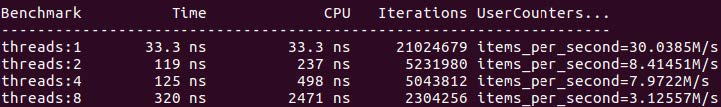
\includegraphics[width=0.9\textwidth]{content/2/chapter7/images/3.jpg}\\
Figure 7.3 – Performance of a mutex-guarded stack
\end{center}

Note that the "item" here is a push followed by a pop, so the value of "items per second" shows how many data elements we can send through the stack every second. For comparison, the same stack without any locks performs more than 10 times faster on a single thread:

\hspace*{\fill} \\ %插入空行
\begin{center}
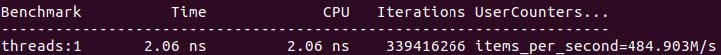
\includegraphics[width=0.9\textwidth]{content/2/chapter7/images/4.jpg}\\
Figure 7.4 – Performance of std::stack (compare with Figure 7.3)
\end{center}

As we can see, the simplest implementation of the stack using a mutex has rather poor performance. However, you should not be in a rush to find or design some clever threadsafe stack, at least not yet. The first question you should ask is, does it matter? What does the application do with the data on the stack? If, say, each data element is a parameter for a simulation that takes several seconds, it probably doesn't matter how fast the stack is. On the other hand, if the stack is at the heart of some real-time transaction processing system, its speed is likely the key to the performance of the entire system.

By the way, the results will likely be similar for any other data structure such as list, deque, queue, and tree, where the individual operations are much faster than the operations on the mutex. But before we can try to improve the performance, we have to consider exactly what kind of performance our application requires.

\subsubsubsection{7.3.3\hspace{0.2cm}Performance requirements for different uses}

For the rest of this chapter, let's assume that the performance of the data structures matters in your application. Now, can we see the fastest stack implementation already? Again, not yet. We also need to consider the use model; in other words, what do we do with the stack and what exactly needs to be fast.

For example, as we have just seen, the key reason for the poor performance of the mutex-guarded stack is that its speed is essentially limited by the mutex itself. Benchmarking the stack operations is almost the same as benchmarking locking and unlocking the mutex. One way to improve the performance would be to improve the implementation of the mutex or use another synchronization scheme. Another way is to use the mutex less often; this way requires that we redesign the client code.

For example, very often, the caller has multiple items that must be pushed onto the stack. Similarly, the caller may be able to pop several elements at once from the stack and process them. In this case, we can implement a batch push or a batch pop using an array or another container to copy multiple elements to and from the stack at once. Since the overhead of locking is large, we can expect that pushing, say, 1,024 elements on the stack with one lock/unlock operation is faster than pushing each one under a separate lock. Indeed, the benchmark shows this to be the case:

\hspace*{\fill} \\ %插入空行
\begin{center}
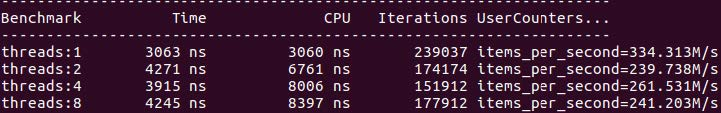
\includegraphics[width=0.9\textwidth]{content/2/chapter7/images/5.jpg}\\
Figure 7.5 – Performance of the batch stack operations (1,024 elements per lock)
\end{center}

We should be very clear about what this technique does and does not accomplish: it reduces the overhead of the locking if the critical section is much faster than the lock operations themselves. It does not make the locked operations scale. Furthermore, by making the critical section longer, we force the threads to wait longer on the lock. This is fine if all threads are mostly trying to access the stack (this is why the benchmark is getting faster). But if, in our application, the threads are mostly doing other computations and only occasionally access the stack, the longer wait will likely degrade the overall performance. To answer definitively whether batch push and batch pop are beneficial, we would have to profile them in a more realistic context.

There are other scenarios where the search for a more limited, application-specific solution can yield performance gains far above what any improved implementation of a general solution can do. For example, this scenario is common in some applications: a single thread pushed a lot of data on the stack upfront, and then multiple threads remove the data from the stack and process it, and maybe push more data onto the stack. In this case, we can implement an unlocked push to be used only in the single-threaded context for the upfront push. While the responsibility is on the caller to never use this method in a multi-threaded context, the unlocked stack is so much faster than the locked one that it may be worth the complexity.

More complex data structures offer a variety of use models, but even the stack can be used by more than simple push and pop. We can also look at the top element without deleting it. The std::stack provides the top() member function, but, once again, it is not transactional, so we have to create our own. It is very similar to the transactional pop() function, only without removing the top element:

\hspace*{\fill} \\ %插入空行
\noindent
\textbf{02\_stack.C}
\begin{lstlisting}[style=styleCXX]
template <typename T> class mt_stack {
	std::stack<T> s_;
	mutable std::mutex l_;
	public:
	std::optional<T> top() const {
		std::lock_guard g(l_);
		if (s_.empty()) {
			return std::optional<T>(std::nullopt);
		} else {
			std::optional<T> res(s_.top());
			return res;
		}
	}
};
\end{lstlisting}

Note that, to allow the lookup-only function, top(), to be declared const, we had to declare the mutex as mutable. This should be done with caution: the convention for multi-threaded programs is that, following the STL, all const member functions are safe to call on multiple threads as long as no non-const member functions are called. This generally implies that const methods do not modify the object, that they are truly read-only. The mutable data members violate this assumption. As a minimum, they should not represent the logical state of the object: they are only implementation details. Then, care should be taken to avoid any race conditions when modifying them. The mutex satisfies both of these requirements.

Now we can consider different use patterns. In some applications, the data is pushed on the stack and popped from it. In others, the top stack element may need to be examined many times between each push and pop. Let's focus on the latter case first. Examine the code for the top() method again. There is an obvious inefficiency here: because of the lock, only one thread can read the top element of the stack at any moment. But reading the top element is a non-modifying (read-only) operation. If all threads did that and no thread tried to modify the stack at the same time, we would not need the lock at all, and the top() operation would scale perfectly. Instead, it has a performance similar to that of the pop() method.

The reason we cannot omit lock in top() is that we cannot be sure that another thread is not calling push() or pop() at the same time. But even then, we do not need to lock two calls to top() against each other; they can proceed simultaneously. Only the operations that modify the stack need to be locked. There is a type of lock that provides such functionality; it is most commonly called a read-write lock. Any number of threads can take the read lock, and these threads do not impede each other. However, the write lock can be taken by only one thread and only if no other thread holds the read lock. In C++, the terminology is different (but the functionality is exactly the same): the reader threads use the shared lock (any number of shared locks on the same mutex can exist at the same time), but the writer threads need the unique lock (only one such lock can exist on a given mutex). An attempt to take the shared lock will block if another thread holds a unique lock already; similarly, an attempt to take the unique lock will block if another thread holds any lock on the same mutex. With the shared mutex, we can implement the stack with exactly the kind of locking we need; the top() method uses the shared lock, so any number of threads can execute it simultaneously, but the push() and pop() methods require the unique lock:

\begin{lstlisting}[style=styleCXX]
template <typename T> class rw_stack {
	std::stack<T> s_;
	mutable std::shared_mutex l_;
	public:
	void push(const T& v) {
		std::unique_lock g(l_);
		s_.push(v);
	}
	std::optional<T> pop() {
		std::unique_lock g(l_);
		if (s_.empty()) {
			return std::optional<T>(std::nullopt);
		} else {
			std::optional<T> res(std::move(s_.top()));
			s_.pop();
			return res;
		}
	}
	std::optional<T> top() const {
		std::shared_lock g(l_);
		if (s_.empty()) {
			return std::optional<T>(std::nullopt);
		} else {
			std::optional<T> res(s_.top());
			return res;
		}
	}
};
\end{lstlisting}

Unfortunately, our benchmark shows that the performance of the call to top() by itself does not scale even with the read-write lock:

\hspace*{\fill} \\ %插入空行
\begin{center}
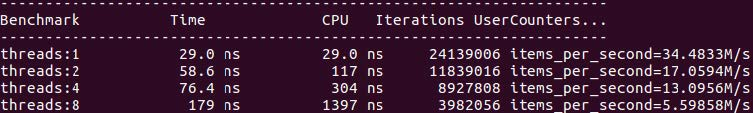
\includegraphics[width=0.9\textwidth]{content/2/chapter7/images/6.jpg}\\
Figure 7.6 – Performance of the stack with std::shared\_mutex; read-only operations
\end{center}

Even worse, the performance of the operations that need the unique lock is degraded even more compared to the regular mutex:

\hspace*{\fill} \\ %插入空行
\begin{center}
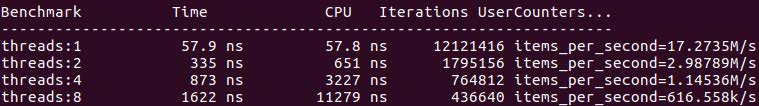
\includegraphics[width=0.9\textwidth]{content/2/chapter7/images/7.jpg}\\
Figure 7.7 – Performance of the stack with std::shared\_mutex; write operations
\end{center}

Comparing Figures 7.6 and 7.7 with the earlier measurements in Figure 7.4, we can see that the read-write lock did not give us any improvement at all. This conclusion is far from universal: the performance of different mutexes depends on the implementation and the hardware. However, in general, the more complex locks, such as the shared mutex, will have more overhead than the simple locks. Their target application is different: if the critical section itself took much longer (say, milliseconds instead of microseconds) and most threads executed read-only code, there would be great value in not locking the read-only threads against each other, and the overhead of a few microseconds would be much less noticeable.

The longer critical section observation is of great importance: if our stack elements were much larger and very expensive to copy, the performance of the locks would matter less compared to the cost of copying the large objects, and we would start to see scaling. However, assuming our overall goal is to make the program fast, rather than showing off a scalable stack implementation, we would optimize the entire application by eliminating the expensive copying altogether and using a stack of pointers instead.

Despite the setback we have suffered with the read-write lock, we are on the right track with the idea of a more efficient implementation. But before we can design one, we have to understand in more detail what exactly each of the stack operations does and what are the possible data races at each step that we must guard against.

\subsubsubsection{7.3.4\hspace{0.2cm}Stack performance in detail}

As we try to improve the performance of the thread-safe stack (or any other data structure) beyond that of the simple lock-guarded implementation, we have to first understand in detail the steps involved in each operation and how they may interact with other operations executed on different threads. The main value of this section is not the faster stack but this analysis: it turns out that these low-level steps are common to many data structures. Let's start with the push operation. Most stack implementations are built on top of some array-like container, so let's view the top of the stack as a contiguous block of memory:

\hspace*{\fill} \\ %插入空行
\begin{center}
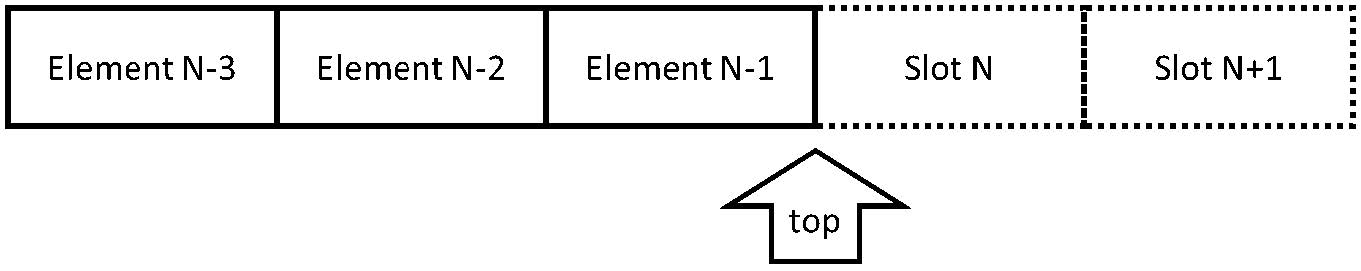
\includegraphics[width=0.9\textwidth]{content/2/chapter7/images/8.jpg}\\
Figure 7.8 – Top of the stack for push operation
\end{center}

There are N elements on the stack, so the element count is also the index of the first free slot where the next element would go. The push operation must increment the top index (which is also the element count) from N to N+1 to reserve its slot and then construct the new element in the slot N. Note that this top index is the only part of the data structure where the threads doing push can interact with each other: as long as the index increment operation is thread-safe, only one thread can see each value of the index. The first thread to execute the push advances the top index to N+1 and reserves the Nth slot, the next thread increments the index to N+2 and reserves the N+1st slot, and so on. The key point here is that there is no race for the slots themselves: only one thread can get a particular slot, so it can construct the object there without any danger of another thread interfering with it.

This suggests a very simple synchronization scheme for the push operations: all we need is a single atomic value for the top index:

\begin{lstlisting}[style=styleCXX]
std::atomic<size_t> top_;
\end{lstlisting}

A push operation atomically increments this index and then constructs the new element in the array slot indexed by the old value of the index:

\begin{lstlisting}[style=styleCXX]
const size_t top = top_.fetch_add(1);
new (&data[top]) Element(… constructor arguments … );
\end{lstlisting}

Again, there is no need to protect the construction step from other threads. The atomic index is all we need to make the push operations thread-safe. By the way, this is true if we use an array as the stack memory. If we use a container such as std::deque, we cannot simply construct a new element over its memory: we have to call push\_back to update the size of the container, and that call is not thread-safe even if the deque does not need to allocate more memory. For this reason, data structure implementations that go beyond basic locks usually also have to manage their own memory. Speaking of memory, we have assumed so far that the array has space to add more elements, and we do not run out of memory. Let's stick with this assumption for now.

What we have so far is a very efficient way to implement a thread-safe push operation in a particular case: multiple threads may be pushing data onto the stack, but nobody is reading it until all push operations are done.

The same idea works if we have a stack with elements already pushed onto it, and we need to pop them (and no more new elements are added). Figure 7.8 works for this scenario as well: a thread atomically decrements the top count and then returns the top element to the caller:

\begin{lstlisting}[style=styleCXX]
const size_t top = top_.fetch_sub(1);
return std::move(data[top]);
\end{lstlisting}

The atomic decrement guarantees that only one thread can access each array slot as the top element. Of course, this works only as long as the stack is not empty. We could change the top element index from an unsigned to a signed integer; then, we would know that the stack is empty when the index becomes negative.

This is, again, a very efficient way to implement thread-safe pop operation under very special conditions: the stack is already populated, and no new elements are added. In this case, we also know how many elements are on the stack, so it is fairly easy to avoid an attempt to pop the empty stack.

In some specific applications, this may be of some value: if the stack is first populated by multiple threads without any pops and there is a clearly defined point in the program where it switches from adding data to removing it, then we have a great solution for each half of the problem. But let's continue to a more general case.

Our very efficient push operation is, unfortunately, of no help when it comes to reading from the stack. Let's consider again how we would implement the operation that pops the top element. We have the top index, but all it tells us is how many elements are currently being constructed; it says nothing about the location of the last element whose construction is completed (element N-3 in Figure 7.9):

\hspace*{\fill} \\ %插入空行
\begin{center}
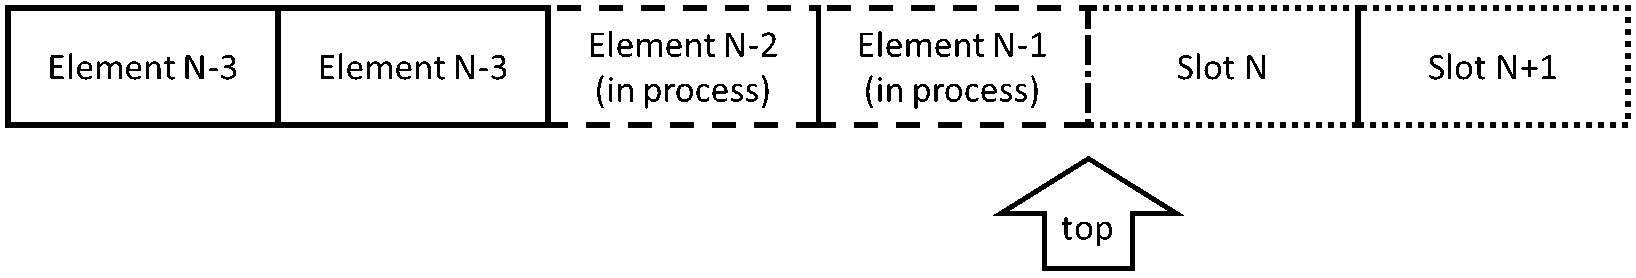
\includegraphics[width=0.9\textwidth]{content/2/chapter7/images/9.jpg}\\
Figure 7.9 – Top of the stack for push and pop operations
\end{center}

Of course, the thread that does the push and, therefore, the construction, knows when it's done. Perhaps what we need is another count that shows how many elements are fully constructed. Alas, if only it was that simple. In Figure 7.9, let's assume that thread A is constructing the element N-2 and that thread B is constructing the element N-1. Obviously, thread A was the first to increment the top index. But it doesn't mean it will also be the first to complete the push. Thread B may finish the construction first. Now, the last constructed element on the stack has the index N-1, so we could advance the constructed count to N-1 (note that we jumped over element N-2, which is still in the middle of the construction). Now we want to pop the top element; no problem, the element N-1 is ready, and we can return it to the caller and remove it from the stack; the constructed count is now decremented to N-2. Which element should we pop next? The element N-2 is still not ready, but nothing in our stack warns us about it. We have only one count for completed elements, and its value is N-1. Now we have a data race between the thread that constructs a new element on the stack and the thread that tried to pop it.

Even without this race, there is another problem: we just popped the element N-1, which was the right thing to do at the time. But while that was happening, a push was requested on thread C. Which slot should be used? If we use slot N-1, we risk overwriting the same element that is currently being accessed by thread A. If we use slot N, then, once all the operations are completed, we have a hole in the array: the top element is N, but the next one is not N-1: it was already popped, and we have to jump over it. Nothing in this data structure tells us that we must do so.

We could keep track of which elements are real and which ones are holes, but this is becoming more and more complex (and doing it in a thread-safe manner will require additional synchronization that will reduce performance). Also, leaving many array slots unused wastes memory. We could attempt to reuse the holes for new elements pushed on the stack, but at this point, the elements are no longer stored consecutively, the atomic top count no longer works, and the whole structure begins to resemble a list. By the way, if you think that a list would be a great way to implement a thread-safe stack, wait until you see what it takes to implement a thread-safe list later in this chapter.

At this point in our design, we must pause the deep dive into the implementation details and again review the more general approach to the problem. There are two steps that we must do: generalize the conclusions from our deeper understanding of the details of the stack implementations and do some performance estimates to get a general idea about what solutions are likely to yield performance improvements. We will start with the latter.

\subsubsubsection{7.3.5\hspace{0.2cm}Performance estimates for synchronization schemes}

Our first attempt at a very simple stack implementation without a lock yielded some interesting solutions for special cases but no general solution. Before we spend much more time building a complex design, we should try to estimate how likely is it that it is going to be more efficient than the simple lock-based one.

Of course, this may seem like circular reasoning: in order to estimate the performance, we must first have something to estimate. But we don't want to do the complex design without at least some assurances that the effort will pay off, the assurances that require a performance estimate.

Fortunately, we can fall back on the general observations we learned earlier: the performance of concurrent data structures depends largely on how many shared variables are accessed concurrently. Let's assume that we can come up with a clever way to implement the stack with a single atomic counter. It is reasonable to assume that every push and pop will have to do at least one atomic increment or decrement of this counter (unless we are doing batch operations, but we already know that they are faster). We can get a reasonable performance estimate if we make a benchmark that combines push and pop on the single-threaded stack with an atomic operation on a shared atomic counter. There is no synchronization going on, so we have to use a separate stack for every thread to avoid race conditions:

\begin{lstlisting}[style=styleCXX]
std::atomic<size_t> n;
void BM_stack0_inc(benchmark::State& state) {
	st_stack<int> s0;
	const size_t N = state.range(0);
	for (auto _ : state) {
		for (size_t i = 0; i < N; ++i) {
			n.fetch_add(1, std::memory_order_release);
			s0.push(i);
		}
		for (size_t i = 0; i < N; ++i) {
			n.fetch_sub(1, std::memory_order_acquire);
			benchmark::DoNotOptimize(s0.pop());
		}
	}
	state.SetItemsProcessed(state.iterations()*N);
}
\end{lstlisting}

Here, st\_stack is a stack wrapper that presents the same interface as our lock-based mt\_stack but without any locks. The real implementation is going to be somewhat slower because the stack top is also shared between threads, but this will give us an estimate from above: it is highly unlikely that any implementation that is actually threadsafe will outperform this artificial benchmark. What do we compare the results to? The benchmark of the lock-based stack in Figure 7.3 shows the performance of the lock-based stack to be between 30M push/pop operations per second on one thread and 3.1M on 8 threads. We also know the baseline performance of the stack without any locks to be about 485M operations per second (Figure 7.4). On the same machine, our performance estimate with a single atomic counter yields these results:

\hspace*{\fill} \\ %插入空行
\begin{center}
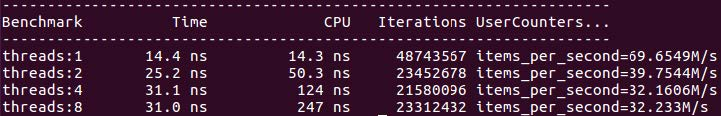
\includegraphics[width=0.9\textwidth]{content/2/chapter7/images/10.jpg}\\
Figure 7.10 – Performance estimate of a hypothetical stack with a single atomic counter
\end{center}

The result seems like a mixed bag: even under optimal conditions, our stack is not going to scale. Again, this is primarily because we are testing a stack of small elements; if the elements were large and expensive to copy, we would see scaling because multiple threads can copy data at the same time. But the earlier observation stands: if copying data becomes so expensive that we need many threads to do it, we are better off using a stack of pointers and not copying any data at all.

On the other hand, the atomic counter is much faster than the mutex-based stack. Of course, this is an estimate from above, but it suggests that a lock-free stack has some possibilities. However, so does the lock-based stack: there are more efficient locks than std::mutex when we need to lock very short critical sections. We had already seen one such lock in Chapter 6, Concurrency and Performance, when we implemented a spinlock. If we use this spinlock in our lock-based stack, then, instead of Figure 7.2, we get these results:

\hspace*{\fill} \\ %插入空行
\begin{center}
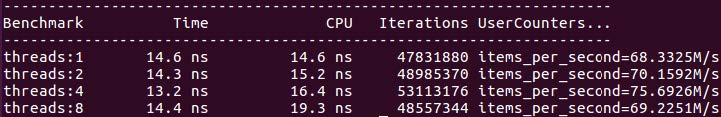
\includegraphics[width=0.9\textwidth]{content/2/chapter7/images/11.jpg}\\
Figure 7.11 – Performance of the spinlock-based stack
\end{center}

Comparing this result with Figure 7.10 paints a very depressing picture: we are not going to come up with a lock-free design that can outperform a simple spinlock. The reason that the spinlock can outperform an atomic increment in some cases has to do with the relative performance of different atomic instructions on this particular hardware; we should not read too much into it.

We could try to do the same estimate with an atomic exchange or compare-and-swap instead of the atomic increment. As you learn more about designing thread-safe data structures, you will get a sense of which synchronization protocol is likely to be useful and what operations should go into the estimate. Also, if you work with particular hardware, you should run simple benchmarks to determine which operations are more efficient on it. All results so far were obtained on X86-based hardware. If we run the same estimates on a large ARM-based server designed specifically for HPC applications, we get a very different outcome. The benchmark of a lock-based stack yields these results:

\hspace*{\fill} \\ %插入空行
\begin{center}
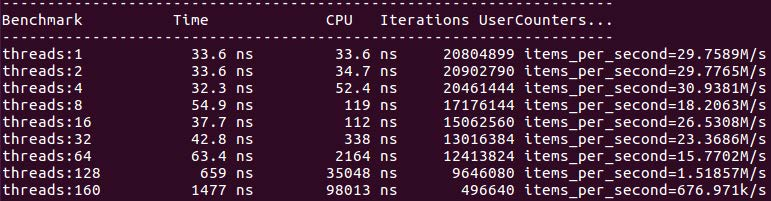
\includegraphics[width=0.9\textwidth]{content/2/chapter7/images/12.jpg}\\
Figure 7.12 – Performance of the lock-based stack on an ARM HPC system
\end{center}

The ARM systems typically have a much larger number of cores than X86 systems, while the performance of a single core is lower. This particular system has 160 cores on two physical processors, and the performance of the lock drops significantly when the program runs on both CPUs. The estimate for the upper limit of the lock-free stack performance should be done with a compare-and-swap instruction instead of the atomic increment (the latter is particularly inefficient on these processors).

\hspace*{\fill} \\ %插入空行
\begin{center}
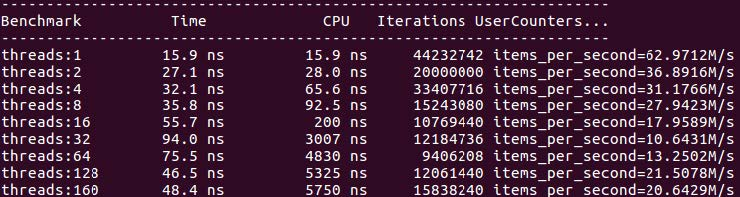
\includegraphics[width=0.9\textwidth]{content/2/chapter7/images/13.jpg}\\
Figure 7.13 – Performance estimate for a hypothetical stack with a single CAS operation (ARM processors)
\end{center}

Based on the estimates in Figure 7.13, there is a chance that, for a large number of threads, we can come up with something better than a simple lock-based stack. We are going to continue with our efforts to develop a lock-free stack. There are two reasons for it: first of all, this effort is ultimately going to pay off on some hardware. Second, the basic elements of this design will be seen later in many other data structures, and the stack offers us a simple test case for learning about them.

\subsubsubsection{7.3.6\hspace{0.2cm}Lock-free stack}

Now that we have decided to try and outperform a simple lock-based implementation, we need to consider the lessons we have learned from our exploration of the push and pop operations by themselves. Each operation is very simple by itself, but the interaction of the two is what creates complexity. This is a very common situation: it is much harder to correctly synchronize producer and consumer operations running on multiple threads than it is to handle only producers or only consumers. Remember this when designing your own data structures: if your application allows for any kind of limitation on the operations you need to support, such as producers and consumers are separate in time, or there is a single producer (or consumer) thread, you can almost certainly design a faster data structure for these limited operations.

Assuming that we need a fully generic stack, the essence of the problem of the producerconsumer interaction can be understood on a very simple example. Again, we assume that the stack is implemented on top of an array or an array-like container, and the elements are stored consecutively. Let's say that we have N elements currently on the stack. The producer thread P is executing the push operation, and the consumer thread C is executing the pop operation at the same time. What should be the outcome? While it is tempting to try to come up with a wait-free design (like we did for only consumers or only producers), any design that allows both threads to proceed without waiting is going to break our fundamental assumption about how the elements are stored: the thread C has to either wait for the thread P to complete the push or return the current top element, N. Similarly, the thread P has to either wait for the thread C to complete or construct a new element in the slot N+1. If neither thread waits, the result is a hole in the array: the last element has the index N+1, but there is nothing stored in the slot N, so we must somehow skip it when we pop data from the stack.

It looks like we have to give up the idea of the wait-free stack implementation and make one of the threads wait for the other one to complete its operation. We also have to deal with the possibility of the empty stack when the top index is zero and a consumer thread attempts to further decrement it. A similar problem occurs at the upper bound of the array when the top index points to the last element and a producer thread needs another slot.

Both of these problems require a bounded atomic increment operation: perform the increment (or decrement) unless the value equals the specified bound. There is no readymade atomic operation for this in C++ (or on any mainstream hardware available today), but we can implement it using compare-and-swap (CAS) as follows:

\begin{lstlisting}[style=styleCXX]
std::atomic<int> n_ = 0;
int bounded_fetch_add(int dn, int maxn) {
	int n = n_.load(std::memory_order_relaxed);
	do {
		if (n + dn >= maxn || n + dn < 0) return -1;
	} while (!n_.compare_exchange_weak(n, n + dn,
			std::memory_order_release,
			std::memory_order_relaxed));
	return n;
}
\end{lstlisting}

This is a typical example of how CAS operation is used to implement a complex lock-free atomic operation:

\begin{enumerate}
\item Read the current value of the variable.
\item Check the necessary conditions. In our case, we verify that the increment would not give us the value outside of the specified bounds [0, maxn). If the bounded increment fails, we signal it to the caller by returning -1 (this is an arbitrary choice; usually, there is a specific action to be performed for the out-of-bounds case).
\item Atomically replace the value with the desired result if the current value is still equal to what we read earlier.
\item If step 3 failed, the current value has been updated, check it again, and repeat steps 3 and 4 until we succeed.
\end{enumerate}

While this may seem to be a kind of lock, there is a fundamental difference: the only way the CAS comparison can fail on one thread is if it succeeded (and the atomic variable was incremented) on another thread, so any time there is a contention for the shared resource, at least one thread is guaranteed to make forward progress.

There is one more important observation that often makes all the difference between a scalable implementation and a very inefficient one. The CAS loop, as written, is very hostile to the scheduling algorithms of most modern operating systems: the thread that loops unsuccessfully also consumes more CPU time and will be given higher priority. This is the exact opposite of what we want: we want the thread that is currently doing the useful work to run faster. The solution is for a thread to yield the scheduler after a few unsuccessful CAS attempts. This is accomplished by a system call that is OS-dependent, but C++ has a system-independent API via the call to std::this\_thread::yield(). On Linux, usually one can get better performance by calling the nanosleep() function to sleep for the minimum possible time (1 nanosecond) every few iterations of the loop:

\begin{lstlisting}[style=styleCXX]
int i = 0;
while ( … ) {
	if (++i == 8) {
		static constexpr timespec ns = { 0, 1 };
		i = 0;
		nanosleep(&ns, NULL);
	}
}
\end{lstlisting}

The same approach can be used to implement much more complex atomic transactions, such as stack push and pop operations. But first, we have to figure out what atomic variables are needed. For the producer threads, we need the index of the first free slot in the array. For the consumer threads, we need the index of the last fully constructed element. This is all the information we need about the current state of the stack, assuming we do not allow "holes" in the array:

\hspace*{\fill} \\ %插入空行
\begin{center}
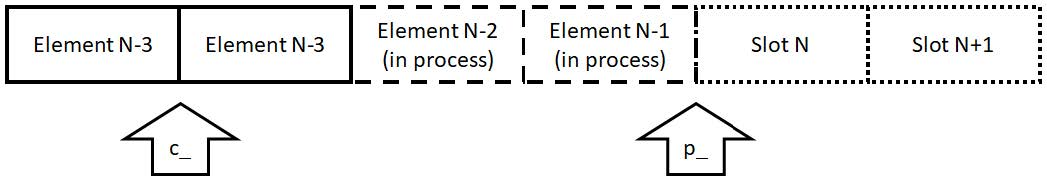
\includegraphics[width=0.9\textwidth]{content/2/chapter7/images/14.jpg}\\ Figure 7.14 – Lock-free stack: c\_ is the index of the last fully constructed element, and p\_ is the index of the first free slot in the array
\end{center}

First of all, neither push nor pop can proceed if the two indices are currently not equal: different counts imply that either a new element is being constructed or the current top element is being copied out. Any stack modification in this state may lead to the creation of holes in the array.

If the two indices are equal, then we can proceed. To do the push, we need to atomically increment the producer index p\_ (bounded by the current capacity of the array). Then we can construct the new element in the slot we just reserved (indexed by the old value of p\_). Then we increment the consumer index c\_ to indicate that the new element is available to the consumer threads. Note that another producer thread could grab the next slot even before the construction is completed, but we would have to wait until all new elements are constructed before we allow any consumer thread to pop an element. Such an implementation is possible, but it is more complex, and it tends to favor the currently executed operation: if a push is currently in progress, a pop has to wait, but another push can proceed without delay. The result is likely to be a swarm of push operations executing while all consumer threads are waiting (the effect is similar if a pop operation is in progress; it favors another pop).

The pop is implemented similarly, only we first decrement the consumer index c\_ to reserve the top slot, and then decrement p\_ after the object is copied or moved from the stack.

There is just one more trick we have to learn, and that is how to manipulate both counts atomically. For example, we said earlier that a thread has to wait for the two indices to become equal. How can this be accomplished? If we read one index atomically and then the other index, also atomically, there is a chance that the first index has changed since we read it. We have to read both indices in a single atomic operation. The same is true for other operations on the indices. C++ allows us to declare an atomic struct of two integers; however, we must be careful: very few hardware platforms have a double CAS instruction that operates on two long integers atomically, and even then, it is usually very slow. The better solution is to pack both values into a single 64-bit word (on a 64-bit processor). The hardware atomic instructions such as load or compare-and-swap do not really care how you are going to interpret the data they read or write: they just copy and compare 64-bit words. You can later treat these bits as a long or a double or a pair of ints (the atomic increment is, of course, different, which is why you cannot use it on a double value).

Now, all that is left is to convert the preceding algorithm into code:

\hspace*{\fill} \\ %插入空行
\noindent
\textbf{02b\_stack\_cas.C}
\begin{lstlisting}[style=styleCXX]
template <typename T> class mt_stack {
	std::deque<T> s_;
	int cap_ = 0;
	struct counts_t {
		int p_ = 0; // Producer index
		int c_ = 0; // Consumer index
		bool equal(std::atomic<counts_t>& n) {
			if (p_ == c_) return true;
			*this = n.load(std::memory_order_relaxed);
			return false;
		}
	};
	mutable std::atomic<counts_t> n_;
	public:
	mt_stack(size_t n = 100000000) : s_(n), cap_(n) {}
	void push(const T& v);
	std::optional<T> pop();
};
\end{lstlisting}

The two indices are 32-bit integers packed into a 64-bit atomic value. The method equal() may look strange, but its purpose will become evident in a moment. It returns true if the two indices are equal; otherwise, it updates the stored index values from the specified atomic variable. This follows the CAS pattern we have seen earlier: if the desired condition is not met, read the atomic variable again.

Note that we can no longer build our thread-safe stack on top of the STL stack: the container itself is shared between threads, and the push() and pop() operations on it are not thread-safe without locking even if the container is not growing. For simplicity, in our example, we used a deque that was initialized with a large enough number of default-constructed elements. As long as we don't call any container member functions, we can operate on different elements of the container from different threads independently. Remember that this is just a shortcut to avoid dealing with memory management and thread safety at the same time: in any practical implementation, you don't want to default-construct all the elements upfront (and the element type may not even have a default constructor). Often, high-performance concurrent software systems have their own custom memory allocators anyway. Otherwise, you can also use an STL container of a dummy type of the same size and alignment as the stack element type, but with a simple constructor and destructor (the implementation is simple enough and is left as an exercise to the reader).

The push operation implements the algorithm we discussed earlier: wait for the indices to become equal, advance the producer index p\_, construct the new object, and advance the consumer index c\_ when done:

\hspace*{\fill} \\ %插入空行
\noindent
\textbf{02b\_stack\_cas.C}
\begin{lstlisting}[style=styleCXX]
void push(const T& v) {
	counts_t n = n_.load(std::memory_order_relaxed);
	if (n.p_ == cap_) abort();
	while (!n.equal(n_) ||
	!n_.compare_exchange_weak(n, {n.p_ + 1, n.c_},
	std::memory_order_acquire,
	std::memory_order_relaxed)) {
		if (n.p_ == cap_) { … allocate more memory … }
	};
	++n.p_;
	new (&s_[n.p_]) T(v);
	assert(n_.compare_exchange_strong(n, {n.p_, n.c_ + 1},
	std::memory_order_release, std::memory_order_relaxed);
}
\end{lstlisting}

The last CAS operation should never fail unless there is a bug in our code: once the calling thread successfully advanced p\_, no other thread can change either value until the same thread advanced c\_ to match (as we already discussed, there is an inefficiency in that, but fixing it comes at the cost of much higher complexity). Also, note that, for brevity, we omitted the call to nanosleep() or yield() inside the loop, but it is essential in any practical implementation.

The pop operation is similar, only it first decrements the consumer index c\_ and then, when it is done removing the top element from the stack, decrements p\_ to match c\_:

\hspace*{\fill} \\ %插入空行
\noindent
\textbf{02b\_stack\_cas.C}
\begin{lstlisting}[style=styleCXX]
std::optional<T> pop() {
	counts_t n = n_.load(std::memory_order_relaxed);
	if (n.c_ == 0) return std::optional<T>(std::nullopt);
	while (!n.equal(n_) ||
		!n_.compare_exchange_weak(n, {n.p_, n.c_ - 1},
			std::memory_order_acquire,
			std::memory_order_relaxed)) {
		if (n.c_ == 0) return std::optional<T>(std::nullopt);
	};
	--n.cc_;
	std::optional<T> res(std::move(s_[n.p_]));
	s_[n.pc_].~T();
	assert(n_.compare_exchange_strong(n, {n.p_ - 1, n.c_},
		std::memory_order_release, std::memory_order_relaxed));
	return res;
}
\end{lstlisting}

Again, the last compare-and-swap should not fail if the program is correct.

The lock-free stack is one of the simplest lock-free data structures possible, and it is already fairly complex. The testing required to validate that our implementation is correct is not straightforward: in addition to all the single-threaded unit tests, we have to validate that there are no race conditions. This task is made much easier by the sanitizer tools such as the Thread Sanitizer (TSAN) available in recent GCC and CLANG compilers. The advantage of these sanitizers is that they detect potential data races, not just the data races that actually happen during the test (in a small test, the chances to observe two threads accessing the same memory incorrectly at the same time are rather slim).

After all our effort, what is the performance of the lock-free stack? As expected, on X86 processors, it does not outperform the spinlock-based version:

\hspace*{\fill} \\ %插入空行
\begin{center}
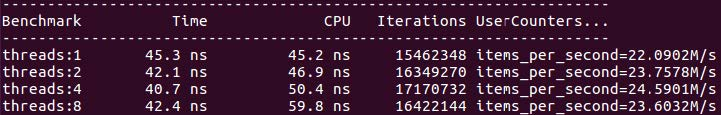
\includegraphics[width=0.9\textwidth]{content/2/chapter7/images/15.jpg}\\ 
Figure 7.15 – Performance of the lock-free stack on X86 CPU (compare with Figure 7.11)
\end{center}

For comparison, the spinlock-guarded stack can execute about 70M operations per second on the same machine. This is consistent with the expectations we had after the performance estimates in the previous section. The same estimates, however, suggested that the lock-free stack may be superior on ARM processors. The benchmark confirms that our efforts were not wasted:

\hspace*{\fill} \\ %插入空行
\begin{center}
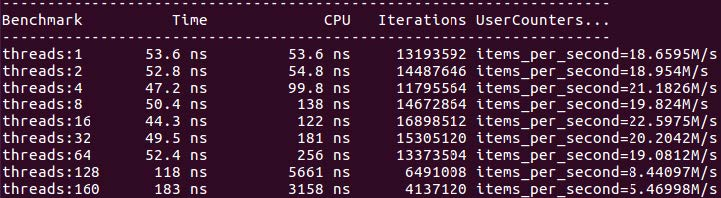
\includegraphics[width=0.9\textwidth]{content/2/chapter7/images/16.jpg}\\ 
Figure 7.16 – Performance of the lock-free stack on ARM CPU (compare with Figure 7.12)
\end{center}

While the single-threaded performance of the lock-based stack is superior, the lock-free stack is much faster if the number of threads is large. The advantage of the lock-free stack becomes even greater if the benchmark includes a large fraction of top() calls (that is, many threads read the top element before one thread pops it) or if the producer and consumer threads are distinct (some threads call only push(), while other threads call only pop()).

To conclude this section, we have explored the different implementations of a thread-safe stack data structure. To understand what is required for thread safety, we had to analyze each operation separately, as well as the interaction of multiple concurrent operations. The following are the lessons that we learned:

\begin{itemize}
\item 
With a good lock implementation, a lock-guarded stack offers reasonable performance and is much simpler than the alternatives.

\item 
Any application-specific knowledge about the limitations on the use of the data structure should be exploited to gain performance cheaply. This is not the place to develop generic solutions, quite the opposite: implement as few features as you can and try to gain performance advantages from the restrictions.

\item 
A generic lock-free implementation is possible but, even for a data structure, that is as simple as a stack, it is quite complex. Sometimes, this complexity may even be justified.

\end{itemize}

So far, we have skirted the issue of memory management: it is hidden behind the vague allocate more memory when the stack runs out of capacity. We will need to come back to that later. But first, let's explore more different data structures.


































